% Written by src/detection/final_figures.py; needs \usepackage{graphicx} and results/figures/ in \graphicspath.
\begin{figure*}[tb]
  \centering
  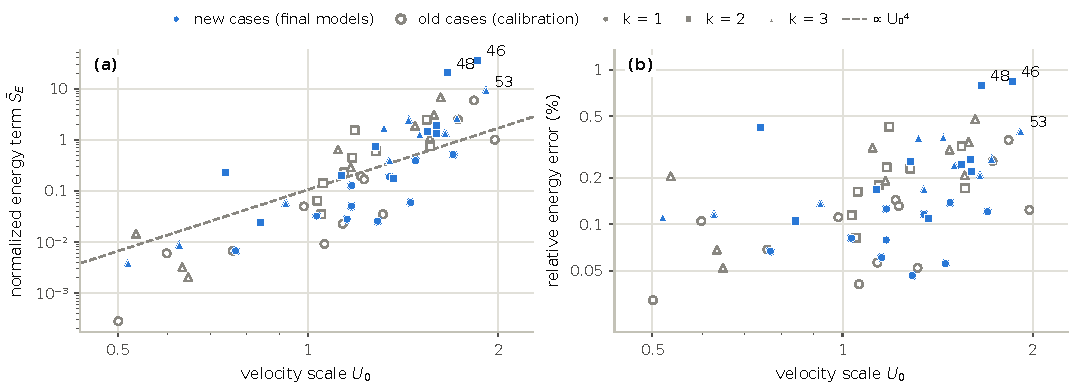
\includegraphics[width=\textwidth]{fig_energy_term_vs_u0.pdf}
  \caption{The energy term of the clean field of each of the 30 new cases (filled) and the 30 old calibration cases (open) against the velocity scale $U_0$ (log axes; marker: $k$). (a) The normalized energy term $\bar S_E$. (b) The relative energy error $\sqrt{S_E}/(U_0^2/4)$: the root-mean-square gap between the model's kinetic energy and its exact decay, over the exact initial energy. $S_E$ is that gap squared in absolute units, so it grows like $U_0^4$ times the squared relative error (dashed line: slope 4). Over the 60 fields the fitted slope is 6.1, steeper, because the relative error itself grows with $U_0$ (Spearman correlation 0.57). Labelled: the new clean fields that Score3 and Score4 flag, case 46, case 48 and case 53 ($U_0$ = 1.86, 1.66 and 1.91), each with a $U_0$ above every old case of its $k$ (old maxima 1.56 for $k = 2$ and 1.62 for $k = 3$).}
  \label{fig:energy_term_vs_u0}
\end{figure*}
